\subsubsection{Minuta de reunião (10-Março-2016)}

\begin{tabbing}
  Local \= xxx \kill
  Local \> : LEAD \\
  Data  \> : 10 de Março de 2016 \\
  Hora  \> : 10:00
\end{tabbing} 

%---------------------------------------------------------------------
\participantes{
  \gabriel,
  \julia,
  \estevão,
  \elael,
  \renan,
  \ramon.

}

\textbf{Aprovação da minuta}

\textbf{Update semanal do Projeto EMMA}

						
\textbf{\gabriel.} 
	\begin{itemize}
			\item Relatório quadrimestral EMMA-METHOD, Metodologia e revestimento
			robótico de turbinas.
			\end{itemize}
		
		\item \textbf{Novas tarefas:}
			\begin{itemize} 
			\item Relatório quadrimestral EMMA-METHOD, Metodologia e revestimento
			robótico de turbinas.
			\end{itemize}

					
   \textbf{\estevão.} 
	\begin{itemize}
		\item \textbf{Tarefas concluídas:}
			\begin{itemize}    
			    \item Detalhamento para orçamento de trilho para testes em laboratório.
				
			\end{itemize}
		
		\item \textbf{Novas tarefas:}
			\begin{itemize} 
			    \item Projeto, detalhamento e orçamento do material para fabricação da pá
			    1:1.
			\end{itemize}
	\end{itemize}

	
	  \textbf{\elael.} 
	\begin{itemize}
		\item \textbf{Tarefas concluídas:}
			\begin{itemize}    
			\item Relatório quadrimestral EMMA-METHOD, Metodologia e revestimento
			robótico de turbinas.
			\end{itemize}
		
		\item \textbf{Novas tarefas:}
			\begin{itemize} 
				\item Relatório quadrimestral EMMA-METHOD, Metodologia e revestimento
				robótico de turbinas.
			\end{itemize}
	\end{itemize}			
			
  \textbf{\renan.} 
	\begin{itemize}
		\item \textbf{Tarefas concluídas:}
			\begin{itemize}    
				\item Relatório quadrimestral EMMA-METHOD, Metodologia e revestimento
				robótico de turbinas.
			\end{itemize}
		
		\item \textbf{Novas tarefas:}
			\begin{itemize} 
				\item Relatório quadrimestral EMMA-METHOD, Metodologia e revestimento
				robótico de turbinas.
			\end{itemize}
	\end{itemize}	
			
   \textbf{\julia.} 
	\begin{itemize}
		\item \textbf{Tarefas concluídas:}
			\begin{itemize}    
				\item Relatório de Interface: Roteiro, introdução e objetivo.
			\end{itemize}
		
		\item \textbf{Novas tarefas:}
			\begin{itemize} 
			    \item Análise do modelo de interação homem-automatização.
			\end{itemize}
	\end{itemize}		




\vspace{5mm}%
\parbox[t]{70mm}{
  Aprovado por: \\[5mm]
  \centering
  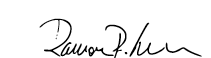
\includegraphics[width=65mm]{figs/logo/assinatura-ramon.png} \\[-4mm]
  \rule[2mm]{70mm}{0.1mm} \\
  \ramon \\[1mm]
  Coordenador do Projeto \\
}

%---------------------------------------------------------------------
\fim